\documentclass[12pt,a4paper]{article}


\usepackage{macros}

\begin{document}\thispagestyle{empty}

\centerline{\Large \bf Homework 7: Due at class on April 25}


 \vspace{.5cm}
\noindent 1. Let us define $S^3=\{(x^0,x^1,x^2,x^3)\in \bR^4 | \sum_{i=0}^3(x^i)^2=1\}$ and $S^1=\{(x^0,x^1,x^2,x^3)\in \bR^4 | (x^0)^2+(x^1)^2=1\}$. Then, show that $S^3 \backslash S^1$ is homotopic to $S^1$.



 \vspace{.5cm}
\noindent 2. Let us identify $S^2 =\bC\cup \{\infty\}$. Then, a holomorphic map $g:\bC\to \bC;z\mapsto z^n$ $(n\in \bZ)$ can be extended to $g:S^2\to S^2$. Find the mapping degree $\deg g$ of $g$.




 \vspace{.5cm}
\noindent 3. \textbf{Fundamental theorem of algebra}

We define $f:\bC\to \bC$  by
$f(z) = z^n +a_1z^{n-1} +\cdots+a_n $ for $n\ge 1$.  In addition, by writing $z=x+iy$, we define one-form
$$
\omega=\textrm{Im}\frac{dz}{z}= \frac{-ydx}{x^2+y^2}+\frac{xdy}{x^2+y^2}~.
$$
Then, show that
$$
\frac{1}{2\pi} \int_{C_R} f^*\omega=n~,
$$
where $C_R$ is the circle with sufficiently large radius $R$. (Hint: construct homotopy between  $f$ and $g$ above.) If there were no zero points $f(z)=0$ inside $C_R$, show that
$$
\frac{1}{2\pi} \int_{C_R} f^*\omega=0~
$$
by using the Stokes theorem.



 \vspace{.5cm}
\noindent 4. Find Poincar\'e dual pairs (non-trivial intersection pairings) in the real-valued homology group $H_{\ell}\left(\Sigma_{g} ; \mathbb{R}\right)$ of a Riemann surface $\Sigma_{g}$ of genus
$g$.

\begin{figure}[ht]\centering
\tikzset{every picture/.style={line width=0.75pt}} %set default line width to 0.75pt

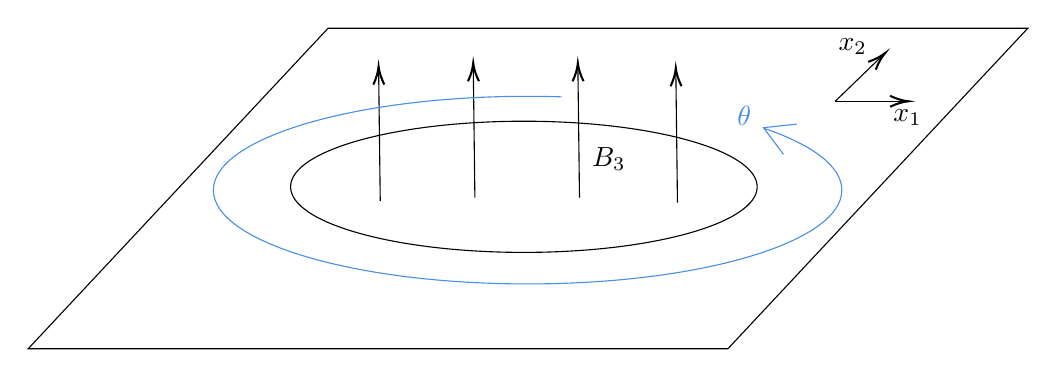
\begin{tikzpicture}[x=0.75pt,y=0.75pt,yscale=-.8,xscale=.8]
%uncomment if require: \path (0,300); %set diagram left start at 0, and has height of 300

%Shape: Ellipse [id:dp5854097192692651]
\draw   (169.5,149.5) .. controls (169.5,127.68) and (232.4,110) .. (310,110) .. controls (387.6,110) and (450.5,127.68) .. (450.5,149.5) .. controls (450.5,171.32) and (387.6,189) .. (310,189) .. controls (232.4,189) and (169.5,171.32) .. (169.5,149.5) -- cycle ;
%Shape: Parallelogram [id:dp9102741300603261]
\draw   (192.1,54) -- (613.5,54) -- (432.9,247) -- (11.5,247) -- cycle ;
%Straight Lines [id:da9933088697414152]
\draw    (223.5,158) -- (222.52,79) ;
\draw [shift={(222.5,77)}, rotate = 449.29] [color={rgb, 255:red, 0; green, 0; blue, 0 }  ][line width=0.75]    (10.93,-3.29) .. controls (6.95,-1.4) and (3.31,-0.3) .. (0,0) .. controls (3.31,0.3) and (6.95,1.4) .. (10.93,3.29)   ;
%Straight Lines [id:da18793371067909592]
\draw    (402.5,159) -- (401.52,80) ;
\draw [shift={(401.5,78)}, rotate = 449.29] [color={rgb, 255:red, 0; green, 0; blue, 0 }  ][line width=0.75]    (10.93,-3.29) .. controls (6.95,-1.4) and (3.31,-0.3) .. (0,0) .. controls (3.31,0.3) and (6.95,1.4) .. (10.93,3.29)   ;
%Straight Lines [id:da3605763006526539]
\draw    (280.5,156) -- (279.52,77) ;
\draw [shift={(279.5,75)}, rotate = 449.29] [color={rgb, 255:red, 0; green, 0; blue, 0 }  ][line width=0.75]    (10.93,-3.29) .. controls (6.95,-1.4) and (3.31,-0.3) .. (0,0) .. controls (3.31,0.3) and (6.95,1.4) .. (10.93,3.29)   ;
%Straight Lines [id:da4503028766714825]
\draw    (343.5,156) -- (342.52,77) ;
\draw [shift={(342.5,75)}, rotate = 449.29] [color={rgb, 255:red, 0; green, 0; blue, 0 }  ][line width=0.75]    (10.93,-3.29) .. controls (6.95,-1.4) and (3.31,-0.3) .. (0,0) .. controls (3.31,0.3) and (6.95,1.4) .. (10.93,3.29)   ;
%Straight Lines [id:da43946037138665517]
\draw    (497.5,98) -- (526.06,70.39) ;
\draw [shift={(527.5,69)}, rotate = 495.97] [color={rgb, 255:red, 0; green, 0; blue, 0 }  ][line width=0.75]    (10.93,-3.29) .. controls (6.95,-1.4) and (3.31,-0.3) .. (0,0) .. controls (3.31,0.3) and (6.95,1.4) .. (10.93,3.29)   ;
%Straight Lines [id:da8474904230806164]
\draw    (497.5,98) -- (539.5,98) ;
\draw [shift={(541.5,98)}, rotate = 180] [color={rgb, 255:red, 0; green, 0; blue, 0 }  ][line width=0.75]    (10.93,-3.29) .. controls (6.95,-1.4) and (3.31,-0.3) .. (0,0) .. controls (3.31,0.3) and (6.95,1.4) .. (10.93,3.29)   ;
%Shape: Arc [id:dp8900654971819639]
\draw  [draw opacity=0] (455.21,114.48) .. controls (484.05,124.39) and (501.5,137.34) .. (501.5,151.5) .. controls (501.5,182.7) and (416.77,208) .. (312.25,208) .. controls (207.73,208) and (123,182.7) .. (123,151.5) .. controls (123,120.3) and (207.73,95) .. (312.25,95) .. controls (319.16,95) and (325.98,95.11) .. (332.7,95.33) -- (312.25,151.5) -- cycle ; \draw  [color={rgb, 255:red, 74; green, 144; blue, 226 }  ,draw opacity=1 ] (455.21,114.48) .. controls (484.05,124.39) and (501.5,137.34) .. (501.5,151.5) .. controls (501.5,182.7) and (416.77,208) .. (312.25,208) .. controls (207.73,208) and (123,182.7) .. (123,151.5) .. controls (123,120.3) and (207.73,95) .. (312.25,95) .. controls (319.16,95) and (325.98,95.11) .. (332.7,95.33) ;
\draw  [color={rgb, 255:red, 74; green, 144; blue, 226 }  ,draw opacity=1 ] (466.35,129.99) -- (454.35,113.89) -- (474.32,111.76) ;

% Text Node

% Text Node
\draw (349.5,124.4) node [anchor=north west][inner sep=0.75pt]    {$B_{3}$};
% Text Node
\draw (531,101.4) node [anchor=north west][inner sep=0.75pt]    {$x_{1}$};
% Text Node
\draw (498,58.4) node [anchor=north west][inner sep=0.75pt]    {$x_{2}$};
% Text Node
\draw (437,99.4) node [anchor=north west][inner sep=0.75pt]    {$\textcolor[rgb]{0.29,0.56,0.89}{\theta }$};



\end{tikzpicture}
\end{figure}

 \vspace{.5cm}
 \noindent 5. (Mapping degree and vortex) Let us consider the $3+1$-dimensional action for a scalar field interacting the electromagnetic field with the potential
$$S=\int d^{4} x\Bigl[-\frac{1}{4} F_{\mu \nu} F^{\mu \nu}+\left|D_{\mu} \phi\right|^{2}-\lambda\left(|\phi|^{2}-v^{2}\right)^{2}\Bigr]$$
with $D_{\mu} \phi=\partial_{\mu} \phi-i A_{\mu} \phi$. Let us consider the situation in which the system is invariant in the $x^{3}$ direction and $A_3 = 0$ so that all the fields depend on the $\left(x^{1}, x^{2}\right)$ plane. We parameterise the plane by the radial coordinates $x^{1}+i x^{2}=r e^{i \theta}$.

\begin{itemize}
  \item Show a necessary condition for  the energy to be finite is that the scalar field configuration $\phi$ is topologically classified by the mapping degree of
  $
 S_{\infty}^{1} \to S^{1}
  $
  at the infinity of the plane. Namely, the configuration is homotomic to $\phi \rightarrow e^{i n \theta} v$ as $r \to \infty$ where $n\in \bZ$.
    \item Compute the Kinetic energy $\int d^{2} x\left|\partial_{i} \phi\right|^{2}$ for this configuration, which is still divergent.
    \item This divergence can be canceled by the gauge potential $A_\mu$. Namely we can have $\int d^{2} x\left|D_{i} \phi\right|^{2}<\infty$ if we choose the gauge potential appropriately. In this case, show that the magnetic flux over the plane is quantized as
    $$
 \frac{1}{2 \pi} \int d^{2} x B_3=n~.
    $$
\end{itemize}


%


 \vspace{.5cm}
\noindent 6.  (This is a bonus problem with extra 3 points which is NOT mandatory.)

Let us consider a non-linear sigma model $S^2\to S^2$. In phyiscs, we usually identify $S^2=\bR^2\cup \{\infty\}$ and we write the action as
$$
S=\frac{1}{4\pi} \int d^2x\left(\frac{1}{2} \partial_{m} X^{i} \partial_{m} X^{i}+2 \lambda\left(X^{i} X^{i}-1\right)^2\right)
$$
where $X:\bR^2\to \bR^3; x\mapsto X(x)$ and $\lambda\in \bR_{>0}$ is the Lagrangian multiplier so that it imposes $|X|^2-1$.
If we define
$$
Q=\frac{1}{8 \pi}\int d^2x \varepsilon^{i j k} \varepsilon_{m n} X^{i} \partial_{m} X^{j} \partial_{n} X^{k}~,
$$
show that $Q$ is an integer and $S\ge Q$. Find a field configuration $X:\bR^2\to \bR^3$ explicitly that saturates the bound $S\ge Q$.







\end{document}
